In this checkpoint, you will implement windowed transmission, where more than one packet can be ``on the wire" at the same time. You will start by extending a simple ``stop and wait" implementation that we provide.

\subsection{Learning Objectives}
With this section, you will learn to think about data packetization and reconstruction, TCP windowing, and packet retransmission. You will also continue to strengthen your C programming skills.

\subsection{Starter Code}
The following files have been provided for you to use:
\begin{itemize}
\item cmu\_packet.h: this file describes the basic packet format and header. You are not allowed to modify this file until the final submission! The scripts that we provide to help you graph your packet traces rely on this file being unchanged.
\item grading.h: these are variables that we will use to test your implementation, please do not make any changes here as we will be replacing it when running tests. 
\item server.c:  this is the starter code for the server side of your transport protocol. 
\item client.c: this is the starter code for the client side of your transport protocol.
\item cmu\_tcp.c: this contains the main socket functions required of your TCP socket including reading, writing, opening and closing. 
\item backend.c: this file contains the code used to emulate the buffering and sending of packets. This is where you should spend most of your time.
gen\_graph.py: Python script that takes in a pcap file and graphs your sequence numbers by time. 
\item cmu\_packet.h
All the communication between your server and client will use UDP as the underlying protocol. All packets will begin with the common header described in cmu\_packet.h as follows:
\begin{itemize}
    \item Course Number 		[4 bytes]
    \item Source Port 			[2 bytes]
    \item Destination Port 		[2 bytes]
    \item Sequence Number 		[4 bytes]
    \item Acknowledgement Number 	[4 bytes]
    \item Header Length		[2 bytes]
    \item Packet Length			[2 bytes]
    \item Flags				[1 byte]
    \item Advertised Window		[2 bytes]
    \item Extension length		[2 bytes]
    \item Extension Data		[You Decide]
\end{itemize}
\end{itemize}

All multi-byte integer fields must be transmitted in network byte order. ntoh, hton, and friends will be very important functions for you to call! All integers must be unsigned, and the course number should be set to 15441 (the scripts rely on this). You are not allowed to change any of the fields in the header, with the exception of the extension data which you may want to modify in Checkpoint 3. Additionally, plen cannot exceed 1400 in order to prevent packets from being broken into parts.

You can verify that your headers are sent correctly using wireshark or tcpdump. You can view packet data sent including the full Ethernet frames. When viewing your packet you should see something similar to the below image; in this case the payload starts at 0x0020. The course number - 15441- shows up in hex as 0x00003C51.\\
  
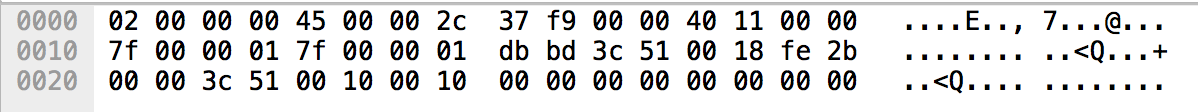
\includegraphics[scale=0.75]{sample_data.png}

\subsection{Checkpoint 1 Tasks }
\begin{enumerate}
    \item TCP Handshakes - Implement TCP start and end handshakes before data transmission starts and ends ~\cite{tcp-conn-state}. This should happen in the constructor and destructor for cmu\_socket. 
    \item Flow Control - You will notice that data transfer is very slow. That is because the starter code is using the Stop-and-Wait algorithm, transmitting one packet at a time! You can do much better by using a window of outstanding packets to send on the network. Extend the implementation to: 1) Change the sequence numbers and ACK numbers to represent the number of bytes sent and received (rather than segments) 2) Implement TCP's sliding window algorithm to send a window of packets and utilize the advertised window to limit the amount of data sent by the sender~\cite{sliding-window}. You do not need to implement Nagle's algortihm.
    \item RTT Estimation -  You will notice that loss recovery is very slow! One reason for this is the starter code uses a fixed retransmission timeout (RTO) of 3 seconds. Implement an adaptive RTO by estimating the RTT with Jacobson/Karels Algorithm or using the Karns/Partridge algorithm~\cite{rto-implementation}. 
    \item Duplicate ACK Retransmission -  Another reason loss recovery is slow is the starter code relies on timeouts to detect packet loss. One way to recover more quickly is to retransmit whenever you see triple duplicate ACKs. Implement retransmission on the receipt of 3 duplicate ACKs.
\end{enumerate}


